% Sine and Cosine functions animation
%
% Author:
% Efraín Soto Apolinar.
% http://www.aprendematematicas.org/
% 
% This animation helps explain the 
% geometric interpretation of the 
% sine and cosine functions.
%

\documentclass[spanish,10pt]{beamer}
%%%<
\usepackage{verbatim}
%%%>

\begin{comment}
:Title: Sine and Cosine functions animation

This animation helps explain the 
geometric interpretation of the 
sine and cosine functions.
\end{comment}


\usepackage[ansinew]{inputenc} % Language = Spanish
%
\usepackage{color}
\usepackage{tikz}
\usepackage{hyperref}
\hypersetup{pdfpagemode=FullScreen}
\usepackage{ifthen}
\usepackage{animate}
%
\usetheme{Warsaw} 
\usecolortheme{whale}
%
%
%
\newcounter{angle}
\setcounter{angle}{0}
%
\begin{document}
%
%
%
\begin{frame}[fragile]{Sine and Cosine functions}
\begin{center}
\begin{animateinline}[loop, poster = first, controls]{30}
%
\whiledo{\theangle<359}{
%
    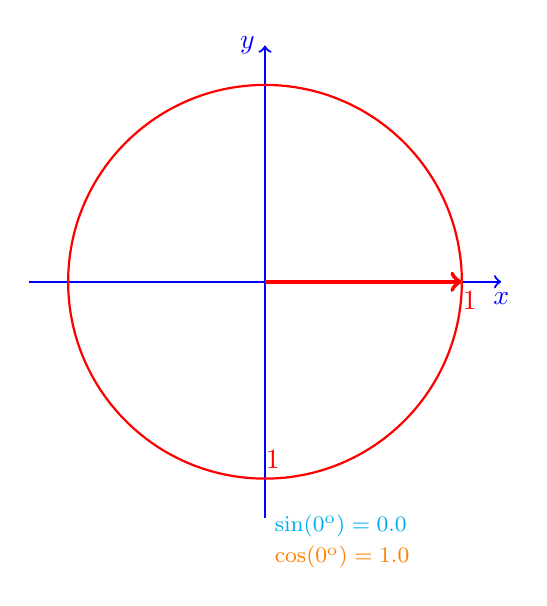
\begin{tikzpicture}
    % Axis
    \draw[thick,->,blue] (-3,0)--(3,0) node[below] {$x$}; % x axis
    \draw[thick,->,blue] (0,-3)--(0,3) node[left] {$y$}; % y axis
    \draw[red,thick] (0,0) circle (2.5cm);
    \node[red,below] at (2.6,0) {1};
    \node[red,above] at (0.1,-2.5) {1};
    %
    \draw[ultra thick,cyan] (0,0) -- (0,0 |- \theangle:2.5cm); % UpOn x axis
    \draw[ultra thick,orange] (0,0) -- (\theangle:2.5cm |- 0,0); % UpOn y axis
    %
    \draw[densely dotted,orange] (\theangle:2.5cm) -- (\theangle:2.5cm |- 0,0); % vertical line
    \draw[densely dotted,cyan] (\theangle:2.5cm) -- (0,0 |- \theangle:2.5cm); % horizontal line
    \draw[ultra thick,red,->,rotate=\theangle] (0,0) -- (2.5,0); 
    \node[red,orange,right] at (0,-3.5) 
            {\footnotesize$\cos(\theangle^{\mathrm{o}}) = \pgfmathcos{\theangle}\pgfmathresult$};
    \node[red,cyan,right] at (0,-3.1) 
            {\footnotesize$\sin(\theangle^{\mathrm{o}}) = \pgfmathsin{\theangle}\pgfmathresult$};
    \end{tikzpicture}
    %
    \stepcounter{angle}
    \ifthenelse{\theangle<359}{
            \newframe
    }{
            \end{animateinline}
    }
}
\end{center}
\end{frame}
%
%
%
\end{document}

